\FloatBarrier
\section{Hauptteil}
\label{sec:haupt:intro}

%\begin{table}[h!]
%	\centering
%	\begin{tabular}{p{0.3\linewidth}|p{0.7\linewidth}}
%		\toprule
%		\textbf{Parameter} & \textbf{Beschreibung} \\ 
%		\midrule
%		$a_1 = 0.05$ & Zuwachsrate der Beutetiere durch Geburten \\
%		\midrule
%		$b_1 = 0.02$ & nat�rliche Todesrate der Beutetiere \\
%		\midrule
%		$c_1 = 0.0006$ & Fressrate der R�uber \\
%		\midrule
%		$a_2 = 0.0002$ & Zuwachsrate der R�uber durch Geburten \\
%		\midrule
%		$b_2 = 0.1$ & nat�rliche Todesrate der R�uber \\
%%		\midrule
%%		$x_{10} = 2500$ & Anfangszahl Beutetiere \\
%%		\midrule
%%		$x_{20} = 10$ & Anfangszahl R�uber \\
%		\bottomrule
%	\end{tabular}
%	\caption{Parameter der Lotka-Volterra-Modelle}
%	\label{tab:haupt:param}
%\end{table}

\subsection{Model \RN{1}: Unbegrenztes Populations-Modell}
\label{sec:haupt:model1}

\subsubsection{Realisierung in MATLAB}
\label{sec:haupt:matlab1}
%Im Folgendem wird erl�utert, wie das Modell 1 der Lotka-Volterra-Gleichungen in MATLAB umgesetzt werden kann. Hierzu erfolgt, in einem ersten Schritt, die Diskretisierung bzw. Ann�herung der Zustandsdifferentialgleichungen aus \autoref{sec:grundl:gl}. Diese kann, basierend auf \cite[S. 262, 296, 532 f.]{lit:Koch2015}, wie folgt definiert werden:

\begin{align}
	\frac{dx}{dt} = \dot{x} &\approx \frac{x_k - x_{k - 1}}{h} \nonumber \\
	x_k &= x_{k - 1} + h \cdotp \dot{x} 
	\label{eqn:haupt:diskret}
\end{align}

\autoref{eqn:haupt:diskret} beschreibt die Linearisierung einer Funktion $x(t)$. Dadurch ist eine Ann�herung der Zustandsgr��en $x_1$ und $x_2$ m�glich. Die momentane �nderung pro Iterationsschritt ist durch $\dot{x}$ gegeben und l�sst sich anhand von \autoref{eqn:grundl:x1} und \autoref{eqn:grundl:x2} berechnen. Die Gr��e $h$ beschreibt die Schrittweite zwischen den Ann�herungen. Diese Ann�herung basiert auf dem Polygonzugverfahren von Euler (vgl. \cite[S. 534]{lit:Koch2015}). Die Beschreibung der kontinuierlichen Gleichungen in diskreter Form erm�glicht und vereinfacht die Implementierung.
\\
\\
Der gesamte MATLAB Code ist hierbei unter \autoref{lst:matlab1:code} gegeben. In einem ersten Schritt m�ssen die Parameter $a_1, b_1, c_1, a_2$ und $b_2$ mit den entsprechenden Anfangswerten deklariert und initialisiert werden. Au�erdem wird eine Maximaldauer $tmax = 50$ Wochen und der entsprechende Zeitschritt $dt = \frac{1}{7}$, der einer �nderung von einem Tag entspricht, festgelegt. Diese k�nnen dazu verwendet werden, um den Zeitvektor $t = \{0, 0+dt, 0+2 \cdot dt, \ldots, tmax-dt, tmax\}$ zu erstellen.

\begin{lstlisting}[style=Matlab-editor,caption={Deklarieren und initialisieren von Parametern},captionpos=b,label=lst:matlab1:param,language=Matlab,basicstyle=\mlttfamily,numbers=none,frame=single,escapeinside={*@}{@*}]
%% Randbedingungen / Parameter [pro Woche]

% Beute / Hasen
a1 = 0.05; % Geburtenrate: Verdopplung der Population in 20 Wochen
b1 = 0.02; % Sterberate: 2% der Hasen sterben an nat�rlichen Ursachen
c1 = 0.0006; % Fressrate der F�chse

% R�uber / F�chse
a2 = 0.0002; % Geburtenrate/Beutewahrscheinlichkeit der F�chse
b2 = 0.1; % Sterberate: F�chse verlieren pro Woche 10% Biomasse

% Anfangsbedingungen
dt = 1/7; % Zeitschritt
tmax = 51*10; % Dauer in Wochen
t = 0:dt:tmax; % Zeitvektor
\end{lstlisting}

Um die bereits genannten Anfangszust�nde abzubilden, werden zwei \emph{for}-Schleifen durchlaufen, in denen $x1$ und $x2$ die entsprechenden Anfangswerte annehmen. Hierbei werden somit sechs verschiedene Anfangszust�nde abgebildet. F�r jede Kombination dieser Anfangswerte wird, f�r jeden Zeitschritt, der entsprechende Wert f�r $x1$ und $x2$ bestimmt. Im ersten Zeitschritt werden hier die Zustandsvariablen mit den entsprechenden Anfangswerten initialisiert. \\In jedem weiteren Zeitschritt wird die �nderung der Beutepopulation $dx1$ sowie R�uberpopulation $dx2$ berechnet. 
\\
\\
Diese werden mit der Schrittweite $h$ multipliziert und auf den $(i - 1)$-ten Wert der Populationen $x1$ und $x2$ addiert, um so den $i$-ten Wert der Zustandsvariablen zu bestimmen. Nach dem Durchlaufen aller Zeitschritte, kann der Verlauf der Populationen grafisch dargestellt werden.
\\
\\
Nach dem Durchlaufen aller Zeitschritte sind alle Werte f�r die Zustandsvariablen berechnet. Diese werden verwendet, um die Verl�ufe der Populationen sowie die dazugeh�rige Phasenkurve darzustellen. Die einzelnen Phasenkurven werden hierbei in einen Plot eingetragen. Dies geschieht durch die Verwendung des Befehls \emph{hold(ax,'on')} bzw. \emph{hold(ax,'off')}.

\begin{lstlisting}[style=Matlab-editor,caption={Berechnen der Verl�ufe und Phasenkurven der Populationen},captionpos=b,label=lst:matlab1:calc,language=Matlab,basicstyle=\mlttfamily,numbers=none,frame=single,escapeinside={*@}{@*}]
% Eigene Axis f�r Phasenkurven
ax = gca;

%% Berechnung
for x20 = [25 10]

for x10 = [2500 1400 650]

	% mit Anfangswerten initialisieren
	x1(1) = x10;
	x2(1) = x20;
	
	for i = 2:length(t)
	
	% �nderung der Beutepopulation
	dx1 = a1*x1(i - 1) - b1*x1(i - 1) - c1*x2(i - 1)*x1(i - 1);
	x1(i) = x1(i - 1) + dt*dx1;
	
	% �nderung der R�uberpopulation
	dx2 = a2*x2(i - 1)*x1(i) - b2*x2(i - 1);
	x2(i) = x2(i - 1) + dt*dx2;
	
	end
	
	figure
	plot(t,x1,t,x2)
	xlabel('Zeit in Wochen','Fontweight','bold')
	ylabel('Population in Stk.','Fontweight','bold')
	legend('Anzahl Beute','Anzahl R�uber')
	set(gca,'Fontweight','bold')
	
	hold(ax,'on')
	plot(ax,x1,x2)
	hold(ax,'off')

end

end

xlabel(ax,'Anzahl Hasen in Stk.','Fontweight','bold')
ylabel(ax,'Anzahl F�chse in Stk.','Fontweight','bold')
title(ax,'Phasenkurve x_2 = f(x_1)')
set(ax,'Fontweight','bold')
\end{lstlisting}

Eine Alternative M�glichkeit, die Phasenkurven zu bestimmen, ist am Ende von \autoref{lst:matlab1:ode} gegeben. Hierzu werden \autoref{eqn:grundl:x1} und \autoref{eqn:grundl:x2} innerhalb einer anonymen Funktion gespeichert, die durch \enquote{@} deklariert wird. Dieser werden die Parameter $t$ und $x$ �bergeben, die entsprechend den Zeitvektor und den Vektor von Zustandsvariablen darstellen. Die Differentialgleichungen, die in dem Function Handle $f$ gespeichert sind, werden numerisch durch den \enquote{ode45}-Solver gel�st bzw. approximiert. Dieser basiert auf dem Runge-Kutta Einschrittverfahren \cite{lit:ode45}. Hierbei wird ein Zeitvektor und bestimmte Anfangswerte an den Solver als Parameter �bergeben. Die Anfangszust�nde werden hierbei mit verschiedenen Faktoren von 0.5 bis 2 multipliziert, um verschiedene Trajektorien abzubilden. Die L�sungswerte in $xs$ enthalten die angen�herten Werte der Zustandsvariablen.

\begin{lstlisting}[style=Matlab-editor,caption={Bestimmung der Phasenkurven durch den ode45-Solver},captionpos=b,label=lst:matlab1:ode,language=Matlab,basicstyle=\mlttfamily,numbers=none,frame=single,escapeinside={*@}{@*}]
figure
hold on
% Zustandsdifferentialgleichungen in anonymer Funktion speichern
f = @(t,x) [x(1)*(a1 - b1 - c1*x(2)); x(2)*(a2*x(1) - b2)];

%Phasenkurven f�r verschiedene Anfangsbedingungen bestimmen
for x20 = [25 10]

for x10 = [2500 1400 650]

	% Verlauf mit ode45 solver berechnen
	[~, xs] = ode45(f,t, [x10, x20]);
	% Phasenkurve plotten
	plot(xs(:,1), xs(:,2))

end

end

xlabel('Anzahl Hasen in Stk.','Fontweight','bold')
ylabel('Anzahl F�chse in Stk.','Fontweight','bold')
title('Phasenkurve x_2 = f(x_1)')
set(gca,'Fontweight','bold')
hold off
\end{lstlisting}

\FloatBarrier

\autoref{img:haupt:mod1_2500_25} bis \autoref{img:haupt:mod1_650_25} zeigen den Verlauf der R�uber- und Beutepopulation f�r $x_{20} = 25$. Hierbei werden f�r $x_{10} = \{2500, 1400, 650\}$ gew�hlt. Es ist zu beobachten, dass die Beutetiere, da sie die einzige Nahrungsquelle der R�uber sind, durch diese aufgezehrt werden.
\\
\\
Aufgrund dessen verringert sich die Beutepopulation rapide. Dieser Verlauf h�lt an, bis die Beutepopulation nicht mehr als Nahrungsquelle f�r die R�uber ausreicht. Dies hat zur Folge, dass sich die Anzahl der R�uber verringert. Durch eine verminderte R�uberpopulation ist es den Beutetieren wieder m�glich, sich zu vermehren. Dieses Wachstum h�lt an, bis die erh�hte Beutepopulation erneut ausreichend f�r die R�uber ist, um sich verst�rkt zu vermehren. Das Verhalten der beiden Populationen wird periodisch wiederholt.
\\
\\
Bei Betrachten der Verl�ufe, f�r die genannten Anfangswerte, hat es den Anschein, dass gr��ere Werte f�r $x_{10}$ und $x_{20}$ in einer h�heren Amplitude und l�ngeren Periode resultieren. F�r $x_{10} = 2500$ und $x_{20} = 25$ ergibt sich, aus \autoref{img:haupt:mod1_2500_25}, eine ungef�hre Periode von ca. 210 Wochen. Dies entspricht einem Zeitraum von ca. vier Jahren. Die Beutetiere erreichen hierbei eine maximale Anzahl von ca. $2500$ wohingegen die R�uber $x_2$ eine maximale Anzahl von ca. $500$ Tieren erreichen. Die Schwankungen der beiden Populationen bewegen sich hierbei, n�herungsweise, zwischen diesen Maximalzahlen.
\\
\\ 
Im Gegensatz dazu bewirken kleinere Anfangswerte $x_{10}$, bei festem $x_{20}$, scheinbar eine geringere Amplitude und Periode. In \autoref{img:haupt:mod1_650_25} ist zu erkennen, dass die Schwankungen der Populationen, f�r $x_{10} = 650$ und $x_{20} = 25$, geringer sind, als f�r $x_{10} = 2500$ und $x_{20} = 25$. Die Anzahl an Beutetieren schwankt hierbei zwischen ca. 300 und 700. Die R�uber schwanken zwischen ca. 25 und 100. Die Periode betr�gt hierbei ca. 150 Wochen. Dies entspricht ca. 3 Jahren.
\\
\\
In \autoref{img:haupt:mod1_2500_10} bis \autoref{img:haupt:mod1_650_10} sind die Verl�ufe der R�uber- und Beutepopulationen f�r $x_{20} = 10$ und $x_{10} = \{2500, 1400, 650\}$ dargestellt. Hierbei sind, f�r die Amplitude und Periodizit�t, �hnliche Aussagen wie f�r \autoref{img:haupt:mod1_2500_25} bis \autoref{img:haupt:mod1_650_25} zu treffen.
\\
\\
Es liegt die Vermutung nahe, dass geringere Anfangswerte f�r $x_1$ und $x_2$ in einer geringeren Amplitude der jeweiligen Population resultiert. Wie die Ergebnisse f�r $x_{10} = 650$ in \autoref{img:haupt:mod1_650_25} bzw. \autoref{img:haupt:mod1_650_10} zeigen, ist dies nicht immer der Fall. Es ist anzumerken, dass die Populationen, f�r beispielsweise $x_{10} = 650$ und $x_{20} = 10$, h�here Schwankungen aufweisen, als f�r $x_{10} = 650$ und $x_{20} = 25$.
\\
\\
Dieses Verhalten ist mit Hilfe der Phasenkurven zu erkl�ren. Diese sind, in \autoref{img:haupt:mod1_phasen}, f�r die Anfangswerte $x_{10} = \{2500, 1400, 650\}$ und $x_{20} = \{25, 10\}$ beispielhaft dargestellt. Hierbei sind in \autoref{img:haupt:mod1_phase} die Verl�ufe der jeweiligen Populationen in der Zustandsebene, auf Basis der mathematischen Beschreibung $x_2 = f(x_1)$, aufgetragen. In \autoref{img:haupt:mod1_phase_ode} sind die, durch den \enquote{ode45}-Solver bestimmten, Phasenkurven dargestellt. Hierbei resultieren die Ungenauigkeiten der Kurven in \autoref{img:haupt:mod1_phase_ode} aus den Ann�herungen, die der \enquote{ode45}-Solver verwendet, um die Zustandsdifferentialgleichungen zu approximieren. Aus den daraus resultierenden Fehlern resultiert eine Abweichung der Phasenkurven, die sich mit der Zeit erh�ht. Die auf dem Polygonzugverfahren von Euler basierende Implementierung in \autoref{lst:matlab1:calc} weist hierbei eine geringere Abweichung �ber der Zeit, als der auf dem Runge-Kutta Verfahren basierende \enquote{ode45}-Solver auf.
\\
\\
Durch den Anfangszustand, der durch $x_{10}$ und $x_{20}$ gegeben ist, verl�uft exakt eine dieser Trajektorien. Diese Trajektorie gibt den Verlauf der Populationen an, der sich, da es sich um geschlossene Kurven handelt, periodisch wiederholt. \\Durch den Umfang der Trajektorien ist die Amplitude des periodischen Verlaufs bzw. die Schwankungen der Populationen zu erkennen. Hierbei ist zu beobachten, dass eine Verringerung der Zustandsvariablen nicht unbedingt in einer geringeren Amplitude resultiert. Es ist ebenso m�glich, dass eine Verringerung der Anfangszust�nde, je nach Lage der Trajektorie, zu einer h�heren Amplitude f�hrt.

\FloatBarrier

\begin{figure}
	\centering
	\begin{subfigure}[h]{0.49\linewidth}
		\centering
		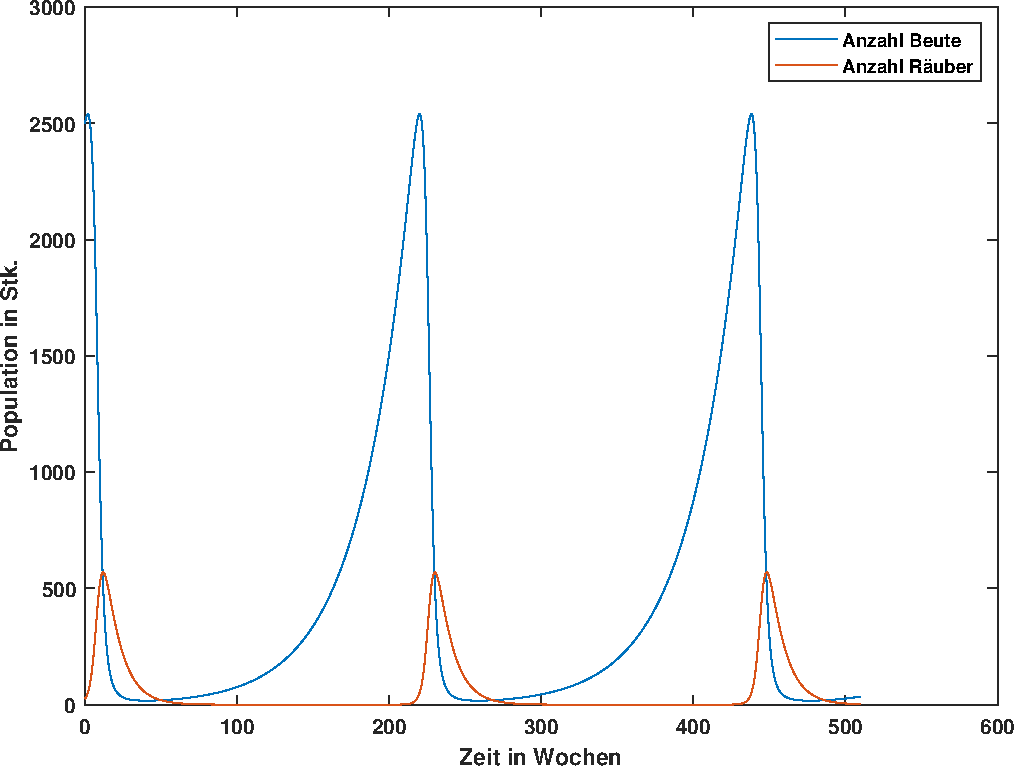
\includegraphics[width=\linewidth,height=0.8\linewidth]{fig/model/Modell1_2500_25}
		\caption{Modell \RN{1} f�r $x_{10} = 2500$ und $x_{20} = 25$}
		\label{img:haupt:mod1_2500_25}
	\end{subfigure}
	\hfill
	\begin{subfigure}[h]{0.49\linewidth}
		\centering
		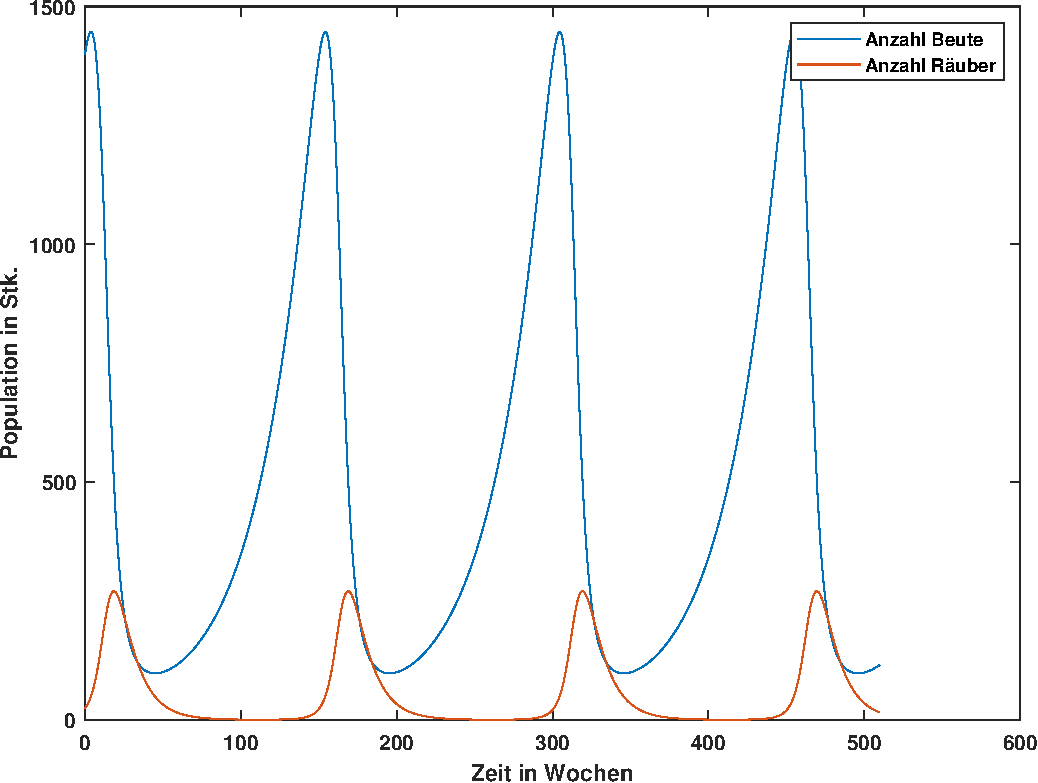
\includegraphics[width=\linewidth,height=0.8\linewidth]{fig/model/Modell1_1400_25}
		\caption{Modell \RN{1} f�r $x_{10} = 1400$ und $x_{20} = 25$}
		\label{img:haupt:mod1_1400_25}
	\end{subfigure}
	\vfill
	\begin{subfigure}[h]{0.49\linewidth}
		\centering
		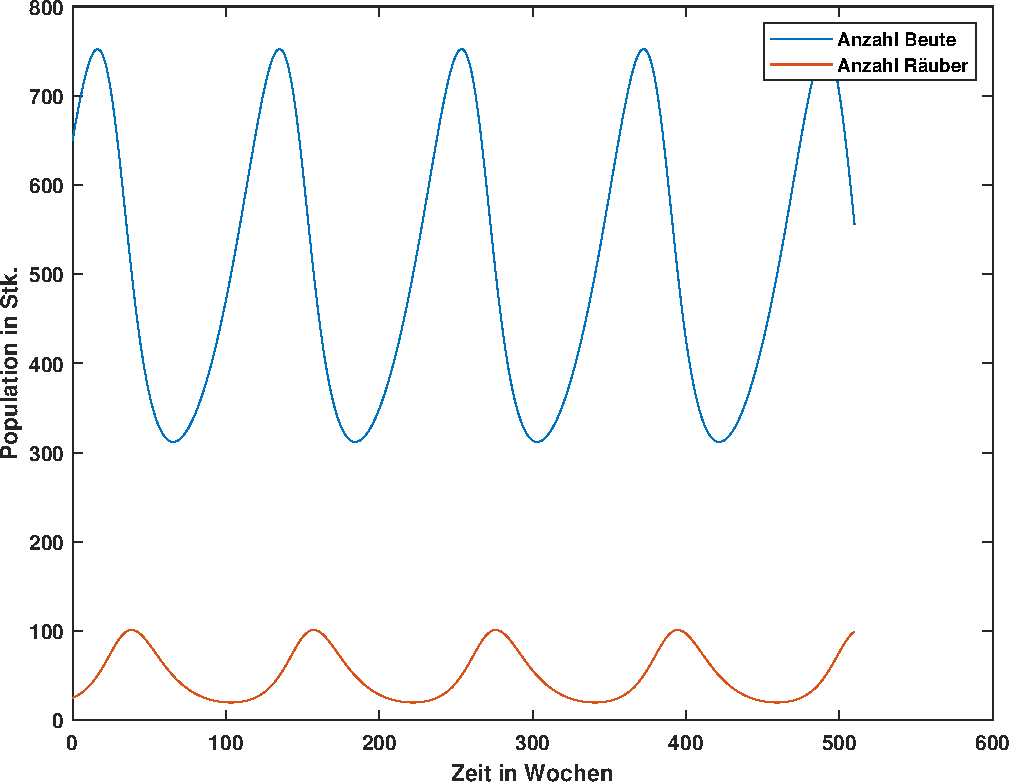
\includegraphics[width=\linewidth,height=0.8\linewidth]{fig/model/Modell1_650_25}
		\caption{Modell 1 f�r $x_{10} = 650$ und $x_{20} = 25$}
		\label{img:haupt:mod1_650_25}
	\end{subfigure}
	\caption{Modell \RN{1} f�r $x_{20} = 25$ und $x_{10} = \{2500, 1400, 650\}$}
	\label{img:haupt:mod1_x10_25}
\end{figure}

\begin{figure}
	\centering
	\begin{subfigure}[h]{0.49\linewidth}
		\centering
		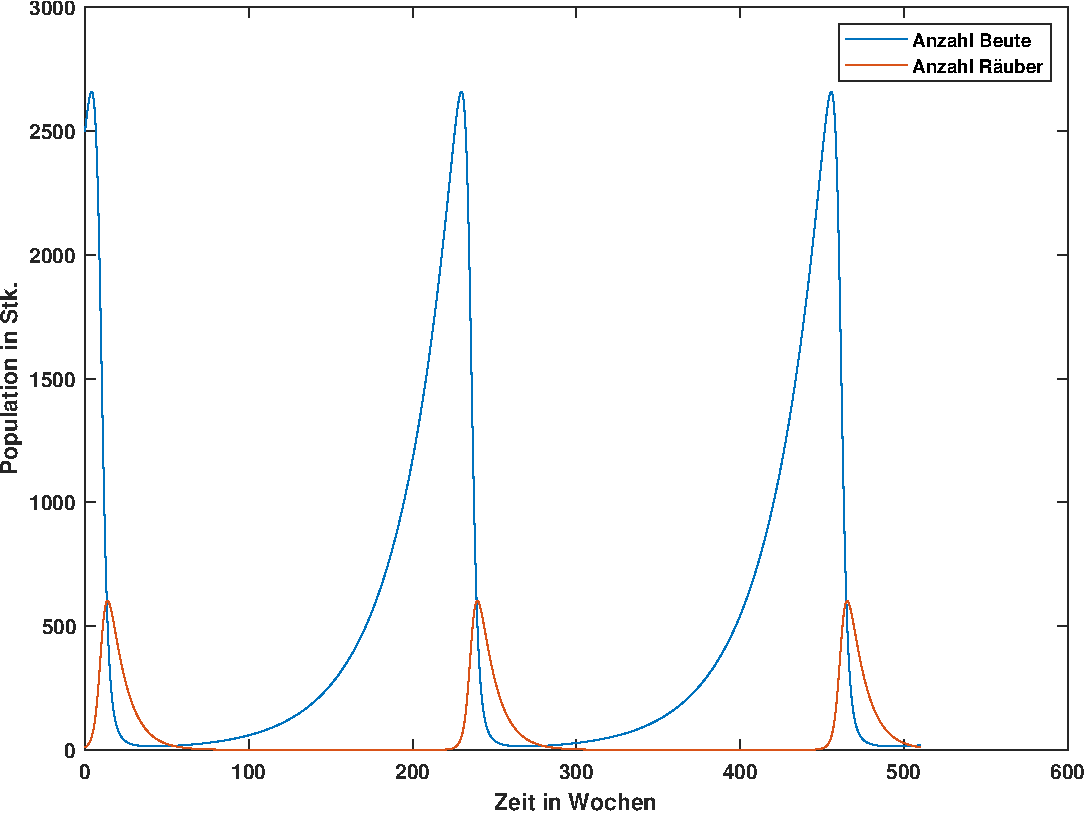
\includegraphics[width=\linewidth,height=0.8\linewidth]{fig/model/Modell1_2500_10}
		\caption{Modell \RN{1} f�r $x_{10} = 2500$ und $x_{20} = 10$}
		\label{img:haupt:mod1_2500_10}
	\end{subfigure}
	\hfill
	\begin{subfigure}[h]{0.49\linewidth}
		\centering
		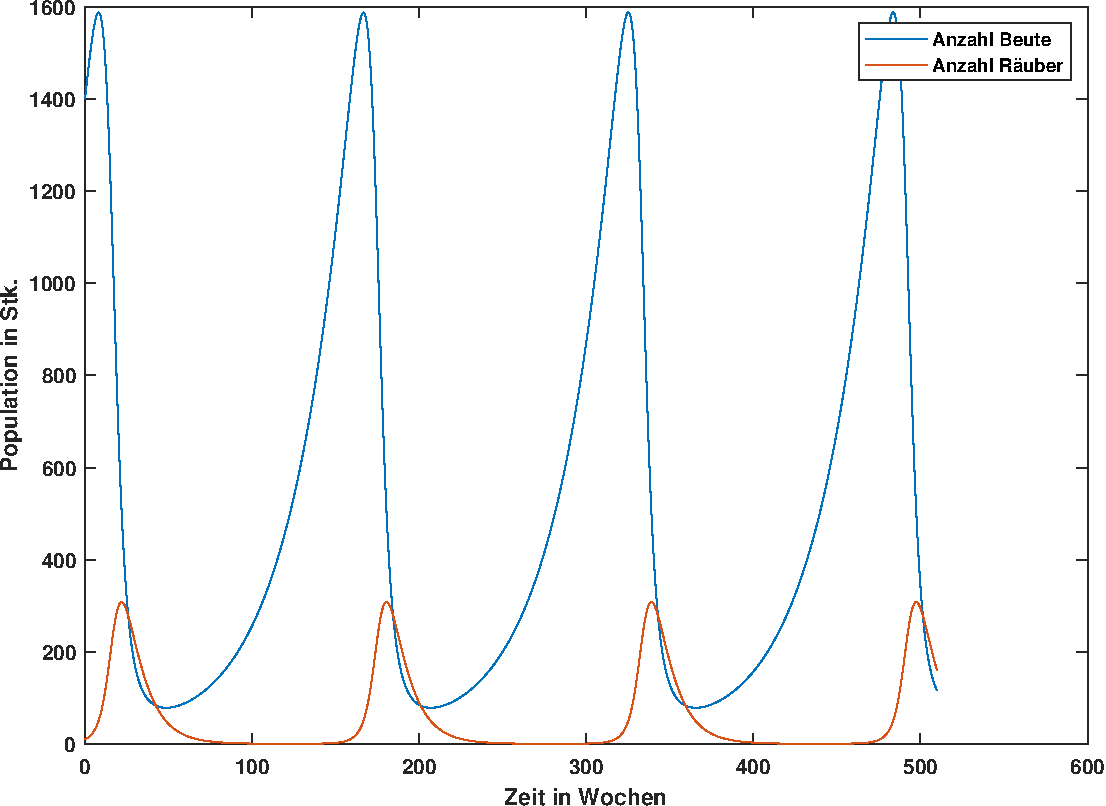
\includegraphics[width=\linewidth,height=0.8\linewidth]{fig/model/Modell1_1400_10}
		\caption{Modell \RN{1} f�r $x_{10} = 1400$ und $x_{20} = 10$}
		\label{img:haupt:mod1_1400_10}
	\end{subfigure}
	\vfill
	\begin{subfigure}[h]{0.49\linewidth}
		\centering
		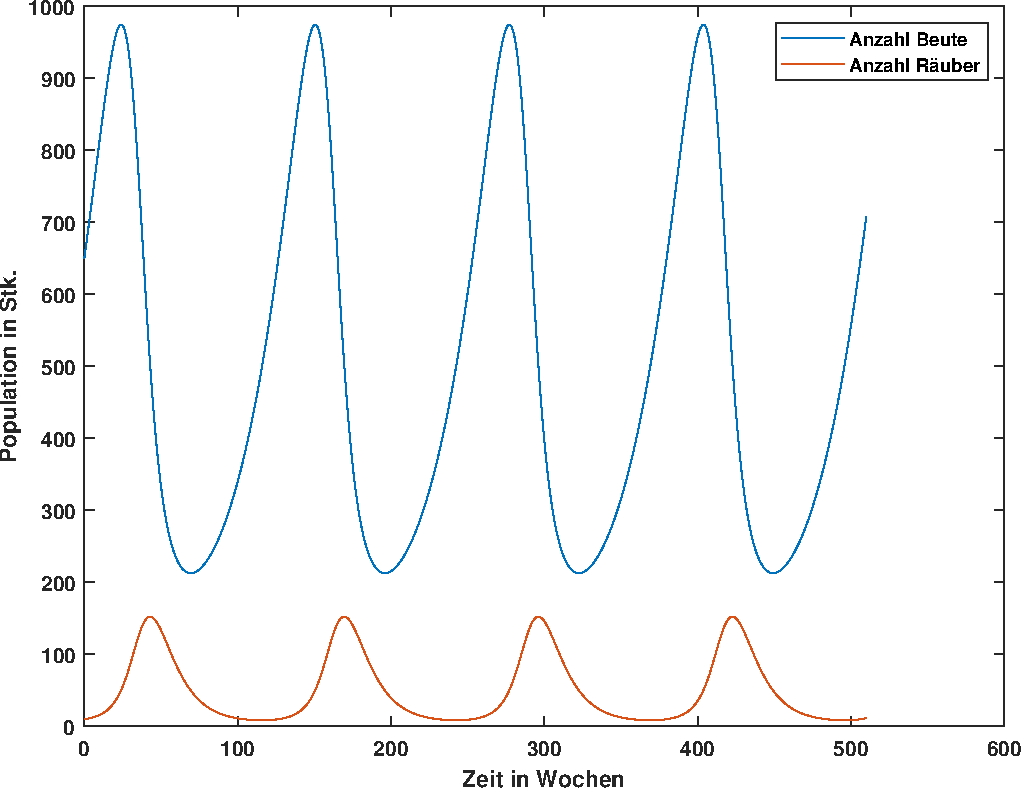
\includegraphics[width=\linewidth,height=0.8\linewidth]{fig/model/Modell1_650_10}
		\caption{Modell \RN{1} f�r $x_{10} = 650$ und $x_{20} = 10$}
		\label{img:haupt:mod1_650_10}
	\end{subfigure}
	\caption{Modell \RN{1} f�r $x_{20} = 10$ und $x_{10} = \{2500, 1400, 650\}$}
	\label{img:haupt:mod1_x10_10}
\end{figure}

\begin{figure}
	\begin{subfigure}[h]{0.49\linewidth}
		\centering
		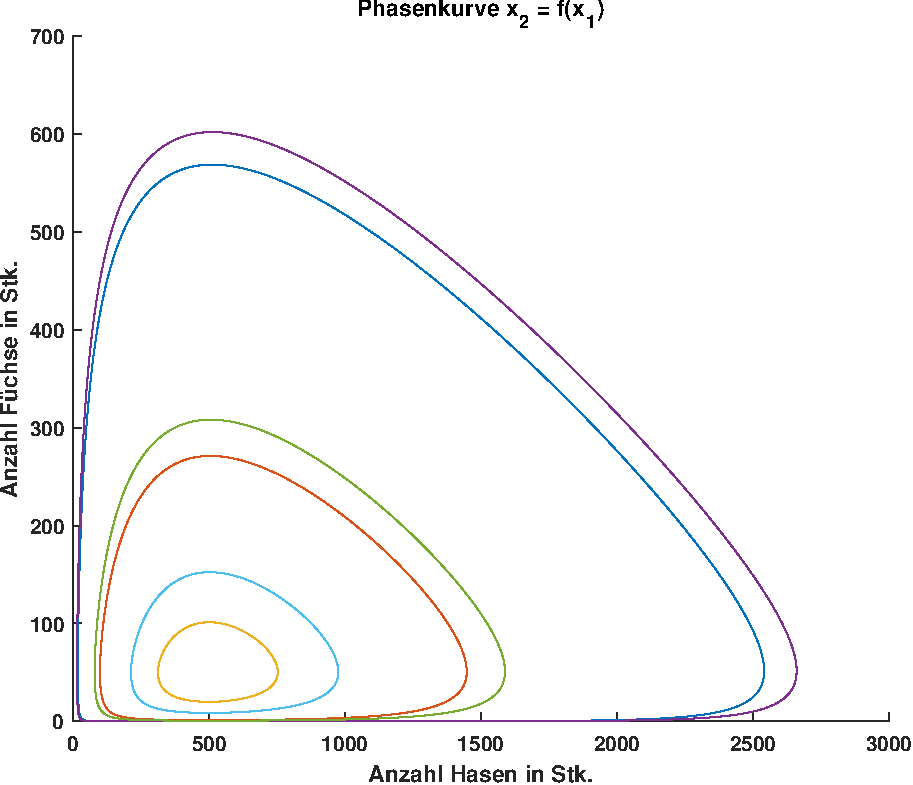
\includegraphics[width=\linewidth,height=0.8\linewidth]{fig/model/Modell1_Phase}
		\caption{Iterativ berechnete Phasenkurven}
		\label{img:haupt:mod1_phase}
	\end{subfigure}
	\hfill
	\begin{subfigure}[h]{0.49\linewidth}
		\centering
		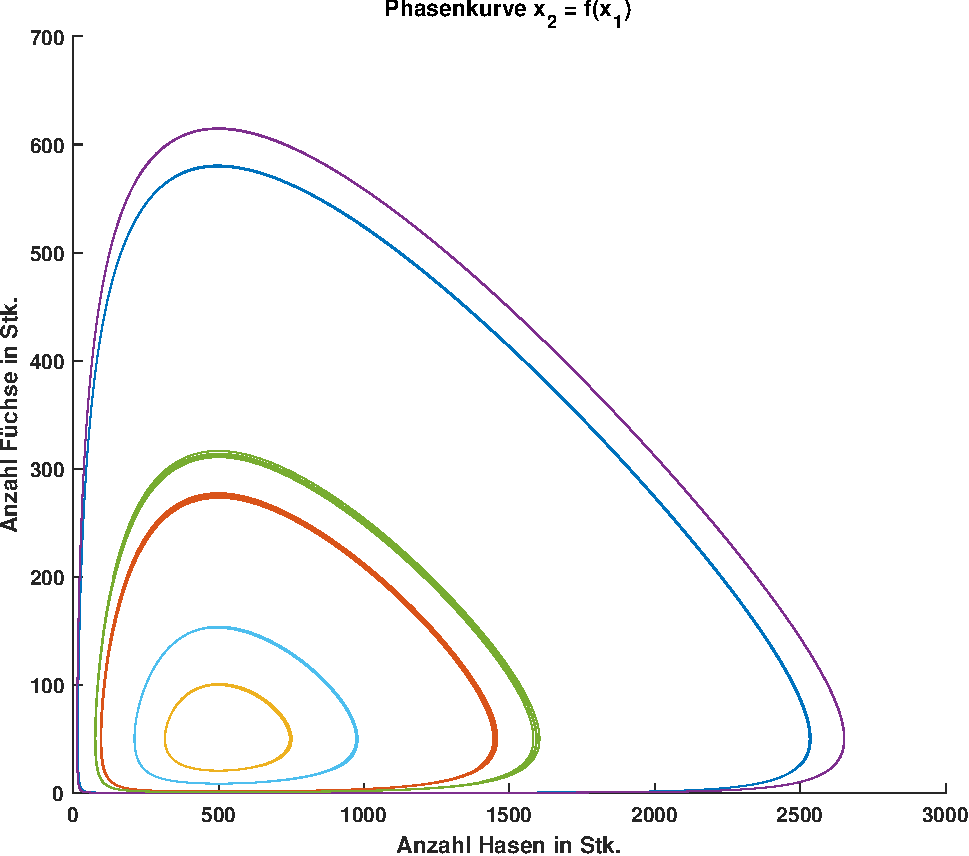
\includegraphics[width=\linewidth,height=0.8\linewidth]{fig/model/Modell1_PhaseOde}
		\caption{Phasenkurven des ode45-Solver}
		\label{img:haupt:mod1_phase_ode}
	\end{subfigure}
	\caption{Phasenkurven $x_2 = f(x_1)$ des Modell \RN{1} f�r verschiedene Anfangswerte}
	\label{img:haupt:mod1_phasen}
\end{figure}

\FloatBarrier

\FloatBarrier
\subsection{Model \RN{2}: Begrenztes Populations-Modell}
\label{sec:haupt:model2}

\subsubsection{Realisierung in MATLAB}
\label{sec:haupt:matlab2}
%Die Realisierung des Modells \RN{2}, unter Verwendung von MATLAB, ist in \autoref{lst:matlab2:code} gegeben. Die Implementierung ist, bis auf spezifische Anpassungen f�r Modell \RN{2}, weitestgehend identisch mit der Realisierung in \autoref{lst:matlab1:code}. Die Parameter $a_1, b_1, c_1, a_2$ und $b_2$ werden in einem ersten Schritt deklariert und initialisiert. Ebenso wird der Zeitvektor $t$, mithilfe der Dauer $tmax$ und dem entsprechenden Zeitschritt $dt$, erstellt. Es wird eine weitere Variable $W$ deklariert und initialisiert, mit der die Weidefl�che bzw. Kapazit�tsgrenze abgebildet werden kann.

\begin{lstlisting}[style=Matlab-editor,caption={Deklarieren und initialisieren von Parametern},captionpos=b,label=lst:matlab2:param,language=Matlab,basicstyle=\mlttfamily,numbers=none,frame=single,escapeinside={*@}{@*}]
%% Randbedingungen / Parameter [pro Woche]

% Beute / Hasen
a1 = 0.05; % Geburtenrate: Verdopplung der Population in 20 Wochen
b1 = 0.02; % Sterberate: 2% der Hasen sterben an nat�rlichen Ursachen
c1 = 0.0006; % Fressrate der F�chse

% R�uber / F�chse
a2 = 0.0002; % Geburtenrate/Beutewahrscheinlichkeit der F�chse
b2 = 0.1; % Sterberate: F�chse verlieren pro Woche 10% Biomasse

% Anfangsbedingungen
W = 1400; % Maximalzahl der Hasen
dt = 1/7; % Zeitschritt
tmax = 51*10; % Dauer in Wochen
t = 0:dt:tmax; % Zeitvektor
\end{lstlisting}

Wie in Modell \RN{1}, werden sechs Anfangszust�nde f�r $x_{10} = \{2500, 1400, 650\}$ und $x_{20} = \{25, 10\}$ in $for$-Schleifen abgebildet. Es wird f�r jeden Zeitschritt die �nderung der Beute- und R�uberpopulation berechnet. Hierbei wird die Berechnung, um die �nderung der Beutepopulation zu bestimmen, an das logistische Wachstum angepasst. Hierzu wird der Term $\frac{W - x1}{W}$ als weiterer Faktor, zur Wachstumsrate $r = a_1 - b_1$, hinzugef�gt.

\begin{lstlisting}[style=Matlab-editor,caption={Berechnen der Verl�ufe und Phasenkurven der Populationen},captionpos=b,label=lst:matlab2:calc,language=Matlab,basicstyle=\mlttfamily,numbers=none,frame=single,escapeinside={*@}{@*}]
% Eigene Axis f�r Phasenkurven
ax = gca;

%% Berechnung

for x20 = [25 10]

for x10 = [2500 1400 650]

	% mit Anfangswerten initialisieren
	x1(1) = x10;
	x2(1) = x20;
	
	for i = 2:length(t)
	
	% �nderung der Beutepopulation mit logistischem Wachstum
	dx1 = 1/W*(W-x1(i - 1))*(a1 - b1)*x1(i - 1) - c1*x2(i - 1)*x1(i - 1);
	x1(i) = x1(i - 1) + dt*dx1;
	
	% �nderung der R�uberpopulation
	dx2 = (a2*x2(i - 1)*x1(i - 1) - b2*x2(i - 1));
	x2(i) = x2(i - 1) + dt*dx2;
	
	end
	
	figure
	plot(t,x1,t,x2)
	xlabel('Zeit in Wochen','Fontweight','bold')
	ylabel('Population in Stk.','Fontweight','bold')
	legend('Anzahl Beute','Anzahl R�uber')
	set(gca,'Fontweight','bold')
	
	hold(ax,'on')
	plot(ax,x1,x2)
	hold(ax,'off')

end

end

xlabel(ax,'Anzahl Hasen in Stk.','Fontweight','bold')
ylabel(ax,'Anzahl F�chse in Stk.','Fontweight','bold')
title(ax,'Phasenkurve x_2 = f(x_1)')
set(ax,'Fontweight','bold')
\end{lstlisting}

Die Phasenkurven lassen sich, ebenso wie f�r das Modell \RN{1}, mit dem \enquote{ode45}-Solver approximieren. Hierzu wird die angepasste \autoref{eqn:haupt:logw} und \autoref{eqn:grundl:x2} in einer anonymen Funktion gespeichert. 

\begin{lstlisting}[style=Matlab-editor,caption={Bestimmung der Phasenkurven durch den ode45-Solver},captionpos=b,label=lst:matlab2:ode,language=Matlab,basicstyle=\mlttfamily,numbers=none,frame=single,escapeinside={*@}{@*}]
figure
hold on
% Zustandsdifferentialgleichungen in anonymer Funktion speichern
f = @(t,x) [x(1)*((a1 - b1)*(1/W*(W - x(1))) - c1*x(2)); x(2)*(a2*x(1) - b2)];

%Phasenkurven f�r verschiedene Anfangsbedingungen bestimmen
for x20 = [25 10]

for x10 = [2500 1400 650]

	% Verlauf mit ode45 solver berechnen
	[~, xs] = ode45(f,t, [x10, x20]);
	% Phasenkurve plotten
	plot(xs(:,1), xs(:,2))

end

end

xlabel('Anzahl Hasen in Stk.','Fontweight','bold')
ylabel('Anzahl F�chse in Stk.','Fontweight','bold')
title('Phasenkurve x_2 = f(x_1)')
set(gca,'Fontweight','bold')
hold off
\end{lstlisting}

\FloatBarrier

Die Verl�ufe der Populationen sind in \autoref{img:haupt:mod2_2500_25} bis \autoref{img:haupt:mod2_650_10} dargestellt. Die entsprechenden Schwankungen der Populationen werden, durch die begrenzte Weidefl�che, ged�mpft. Es ist zu beobachten, dass beide Populationen gegen jeweils einen bestimmten Endwert konvergieren. Dieser ist unabh�ngig von den entsprechenden Anfangszust�nden. Hierauf wird in \autoref{sec:haupt:stationaer} n�her eingegangen. Es ist ebenfalls zu beobachten, dass die Beutepopulation f�r $x_1 \geq W$ rapide abf�llt. Hierbei ist die Kapazit�tsgrenze der Weidefl�che erreicht und es stehen nicht genug Ressourcen f�r alle Beutetiere zur Verf�gung. F�r den Fall $x_{10} = 650$ und $x_{20} = 10$ in \autoref{img:haupt:mod2_650_10} ist, da hierbei $x_1 < W$ gilt, ein Wachstum der Beutepopulation m�glich und zu verzeichnen.
\\
\\
Die Phasenkurven der Anfangszust�nde $x_{10} = \{2500, 1400, 650\}$ und $x_{20} = \{25, 10\}$ f�r das Modell \RN{2} sind in \autoref{img:haupt:mod2_phasen} dargestellt. Hierbei sind keine wesentlichen Unterschiede zwischen der iterativen Berechnung der Phasenkurven und der Bestimmung durch den \enquote{ode45}-Solver zu verzeichnen. Im Gegensatz zu den Phasenkurven f�r das Modell \RN{1} in \autoref{img:haupt:mod1_phase} ist es schwieriger genauere Aussagen �ber den Einfluss der Anfangszust�nde zu machen. Der Verlauf der Phasenkurven ist hierbei wesentlich komplexer. Es ist jedoch das Konvergenzverhalten aller Phasenkurven in Richtung eines station�ren Zustands anzumerken, der unabh�ngig von den Anfangszust�nden ist.

\begin{figure}
	\centering
	\begin{subfigure}[h]{0.49\linewidth}
		\centering
		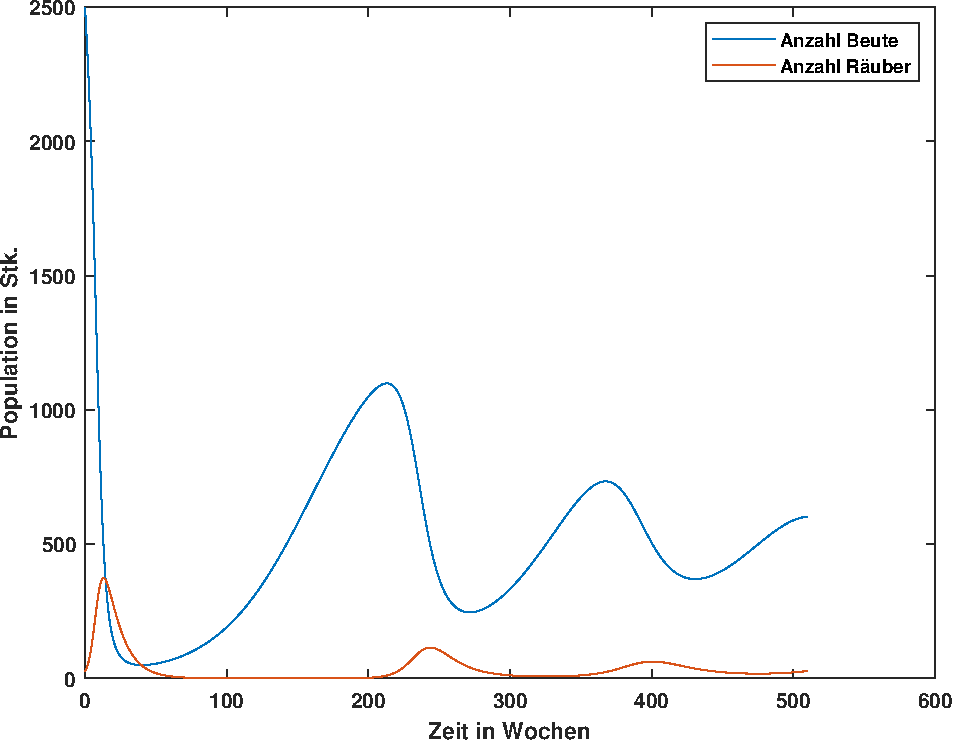
\includegraphics[width=\linewidth,height=0.8\linewidth]{fig/model/Modell2_2500_25}
		\caption{Modell \RN{2} f�r $x_{10} = 2500$ und $x_{20} = 25$}
		\label{img:haupt:mod2_2500_25}
	\end{subfigure}
	\hfill
	\begin{subfigure}[h]{0.49\linewidth}
		\centering
		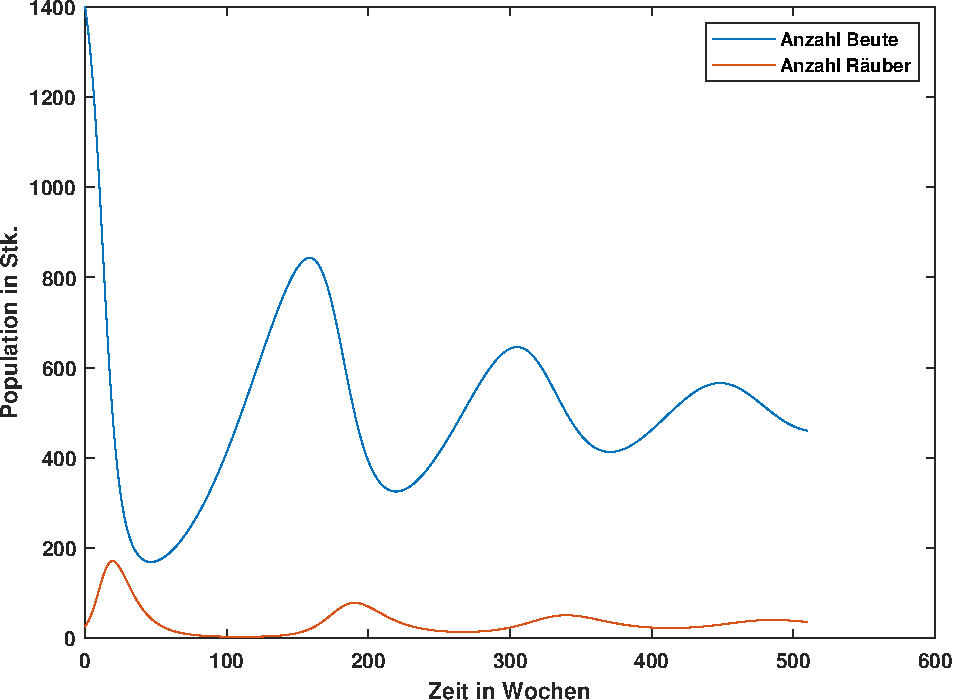
\includegraphics[width=\linewidth,height=0.8\linewidth]{fig/model/Modell2_1400_25}
		\caption{Modell \RN{2} f�r $x_{10} = 1400$ und $x_{20} = 25$}
		\label{img:haupt:mod2_1400_25}
	\end{subfigure}
	\vfill
	\begin{subfigure}[h]{0.49\linewidth}
		\centering
		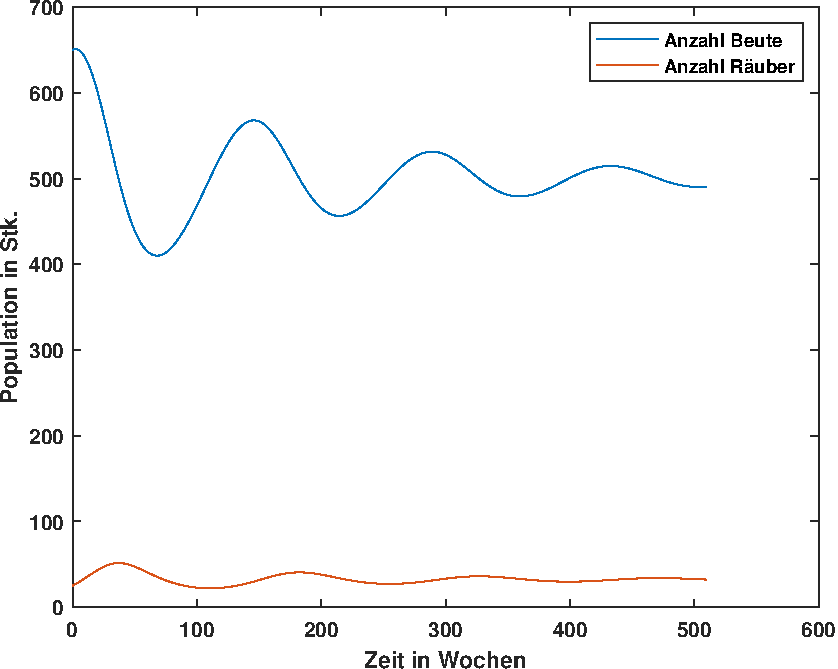
\includegraphics[width=\linewidth,height=0.8\linewidth]{fig/model/Modell2_650_25}
		\caption{Modell 2 f�r $x_{10} = 650$ und $x_{20} = 25$}
		\label{img:haupt:mod2_650_25}
	\end{subfigure}
	\caption{Modell \RN{2} f�r $x_{20} = 25$ und $x_{10} = \{2500, 1400, 650\}$}
	\label{img:haupt:mod2_x10_25}
\end{figure}

\begin{figure}
	\centering
	\begin{subfigure}[h]{0.49\linewidth}
		\centering
		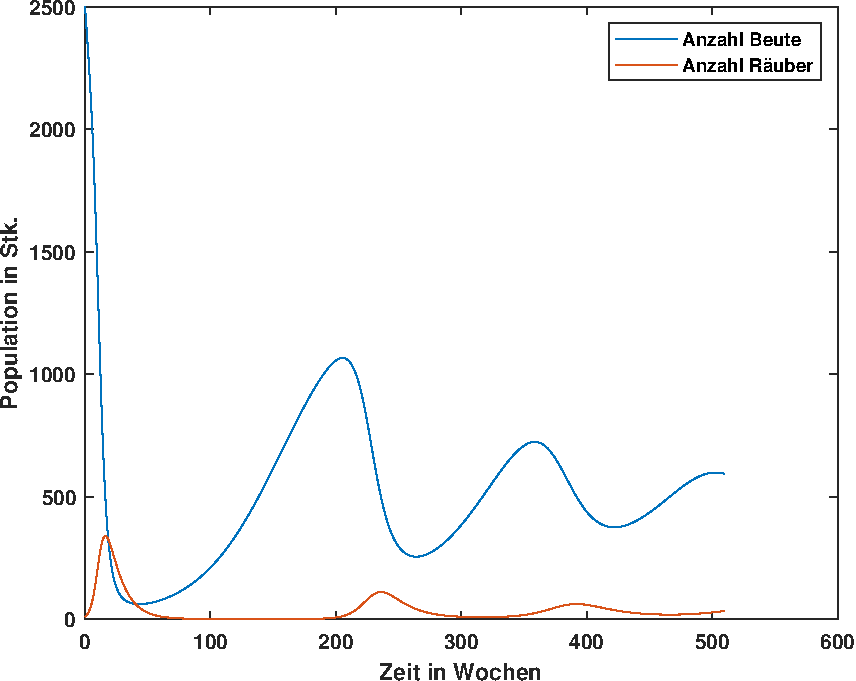
\includegraphics[width=\linewidth,height=0.8\linewidth]{fig/model/Modell2_2500_10}
		\caption{Modell \RN{2} f�r $x_{10} = 2500$ und $x_{20} = 10$}
		\label{img:haupt:mod2_2500_10}
	\end{subfigure}
	\hfill
	\begin{subfigure}[h]{0.49\linewidth}
		\centering
		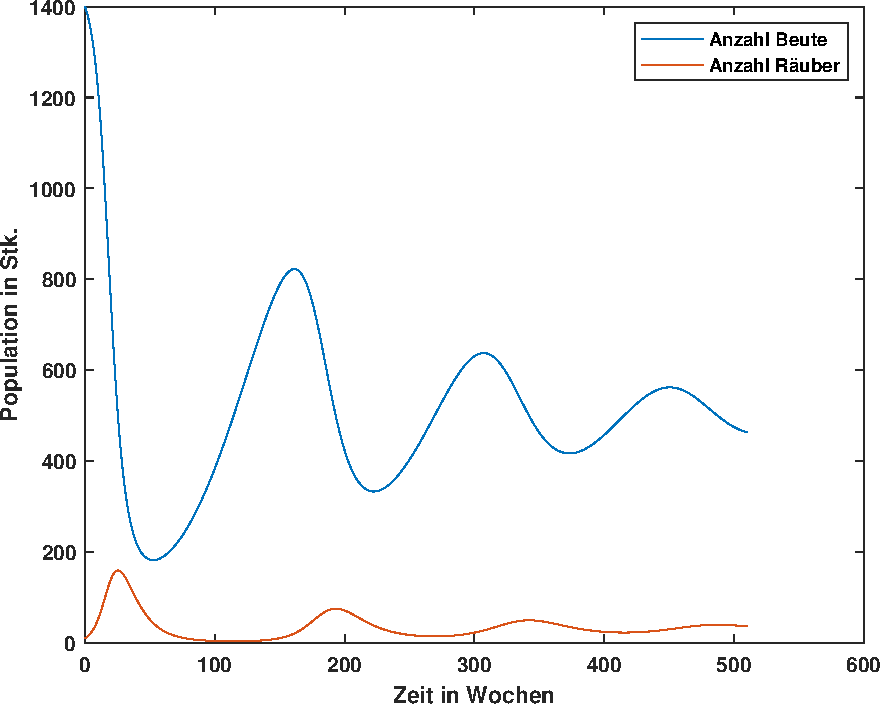
\includegraphics[width=\linewidth,height=0.8\linewidth]{fig/model/Modell2_1400_10}
		\caption{Modell \RN{2} f�r $x_{10} = 1400$ und $x_{20} = 10$}
		\label{img:haupt:mod2_1400_10}
	\end{subfigure}
	\vfill
	\begin{subfigure}[h]{0.49\linewidth}
		\centering
		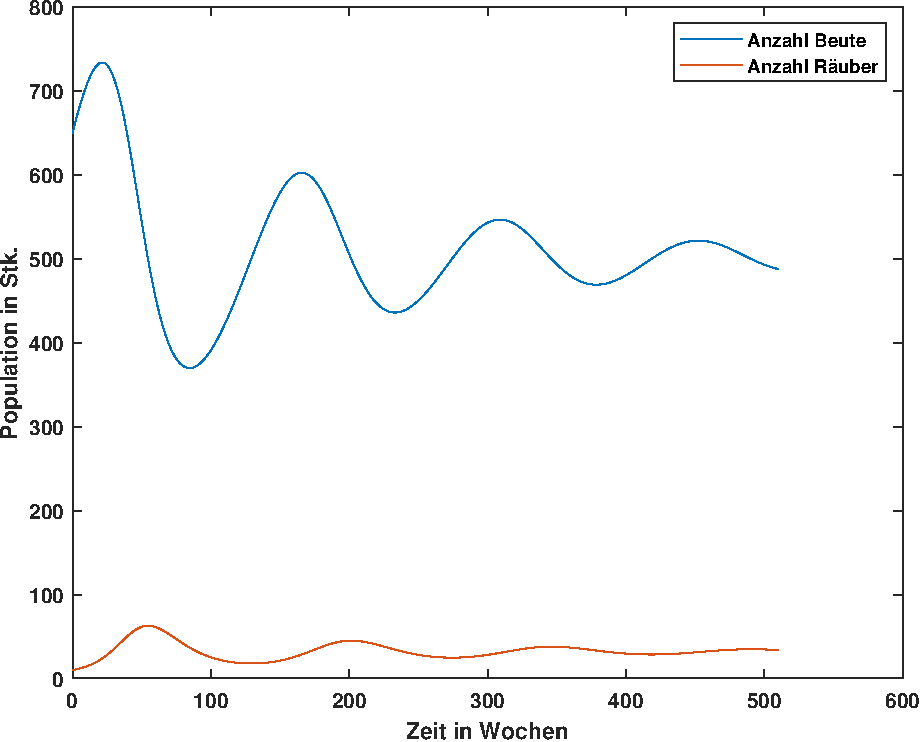
\includegraphics[width=\linewidth,height=0.8\linewidth]{fig/model/Modell2_650_10}
		\caption{Modell \RN{2} f�r $x_{10} = 650$ und $x_{20} = 10$}
		\label{img:haupt:mod2_650_10}
	\end{subfigure}
	\caption{Modell \RN{2} f�r $x_{20} = 10$ und $x_{10} = \{2500, 1400, 650\}$}
	\label{img:haupt:mod2_x10_10}
\end{figure}


\begin{figure}
	\begin{subfigure}[h]{0.49\linewidth}
		\centering
		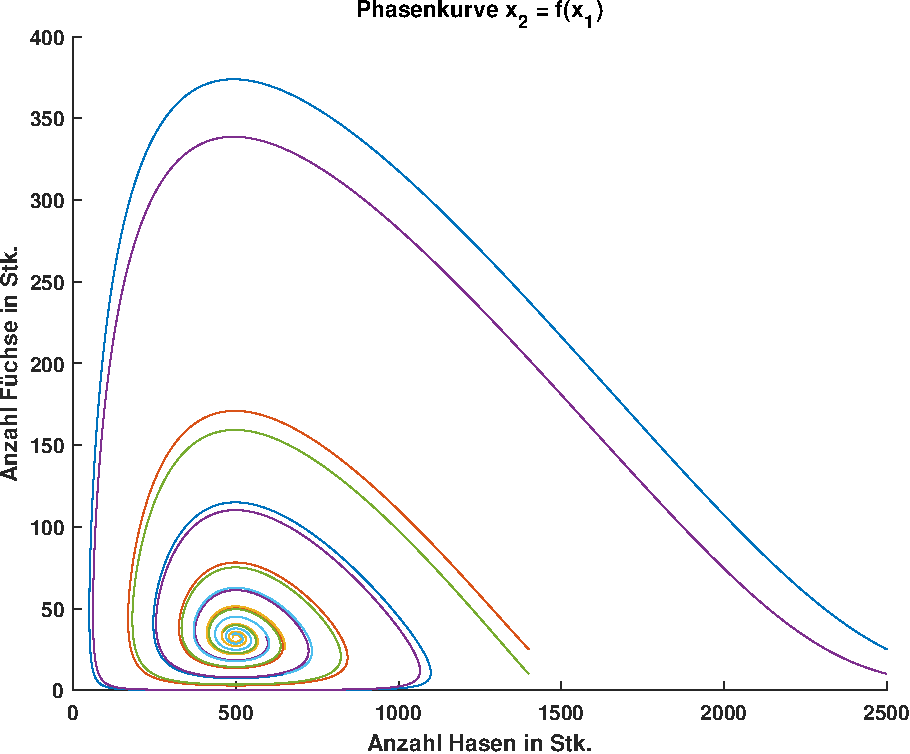
\includegraphics[width=\linewidth,height=0.8\linewidth]{fig/model/Modell2_Phase}
		\caption{Iterativ berechnete Phasenkurven}
		\label{img:haupt:mod2_phase}
	\end{subfigure}
	\hfill
	\begin{subfigure}[h]{0.49\linewidth}
		\centering
		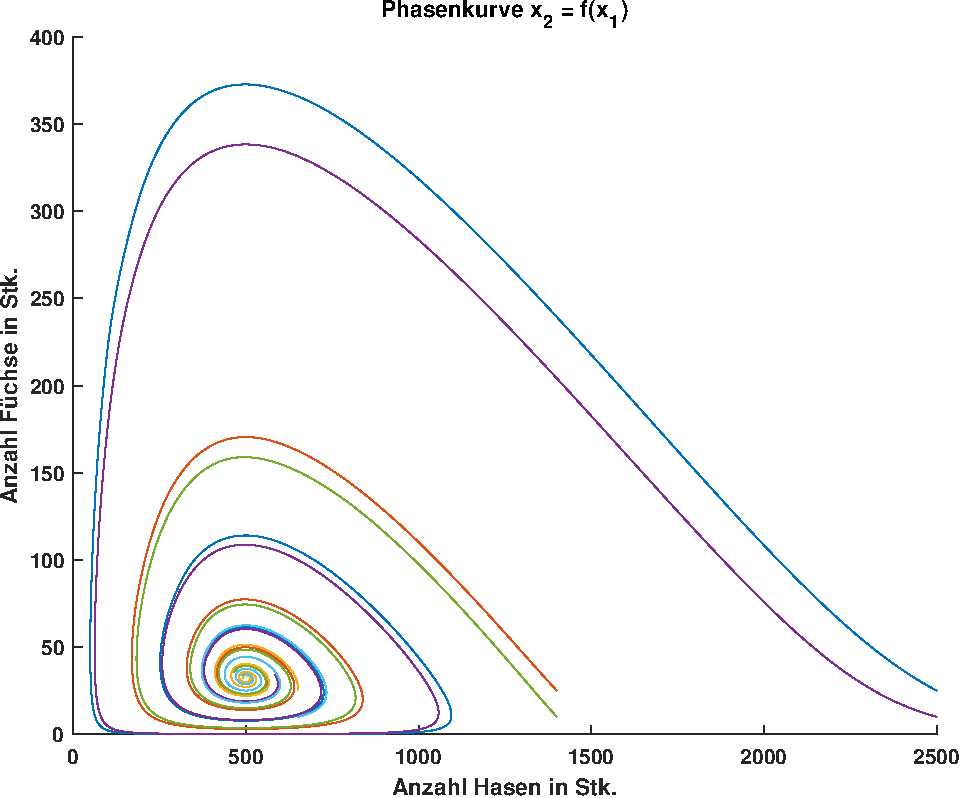
\includegraphics[width=\linewidth,height=0.8\linewidth]{fig/model/Modell2_PhaseOde}
		\caption{Phasenkurven des ode45-Solver}
		\label{img:haupt:mod2_phase_ode}
	\end{subfigure}
	\caption{Phasenkurven $x_2 = f(x_1)$ des Modell \RN{2} f�r verschiedene Anfangswerte}
	\label{img:haupt:mod2_phasen}
\end{figure}

\FloatBarrier

\FloatBarrier
\subsection{Experimente}
\label{sec:haupt:experimente}

\subsubsection{Ermittlung des station�ren Zustands}
\label{sec:haupt:stationaer}
%F�r das Modell \RN{2} war ein Konvergenzverhalten der Populationen zu beobachten. Diese konvergieren in Richtung eines station�ren Zustands. Sie werden auch als Ruhe- bzw. Gleichgewichtslagen $G$, des Lotka-Volterra-Modells, bezeichnet. Sie sind dadurch charakterisiert, dass keine zeitlichen Ver�nderungen der Zustandsvariablen mehr stattfinden \cite[S. 32]{lit:Foellinger1982}:

\begin{align*}
	\dot{x}_1 = 0, \qquad \dot{x}_2 = 0
\end{align*}

Damit folgt aus \autoref{eqn:grundl:x1} und \autoref{eqn:grundl:x2} \cite[S. 32]{lit:Foellinger1982}:

\begin{align}
	(a_1 - b_1 - c_1x_2)x_1 &= 0 
	\label{eqn:haupt:statx1} \\
	(a_2x_1 - b_2)x_2 &= 0
	\label{eqn:haupt:statx2}
\end{align}

Daraus ergibt sich zun�chst die triviale L�sung

\begin{align*}
	x_1 = 0, \qquad x_2 = 0
\end{align*}

in dem die R�uber sowie die Beute ausgestorben sind. Um den weiteren station�ren Zustand der Populationen zu bestimmen, m�ssen die beiden Ausdr�cke in den Klammern in \autoref{eqn:haupt:statx1} und \autoref{eqn:haupt:statx2} null werden \cite[S. 33]{lit:Foellinger1982}:

\begin{align}
	a_1 - b_1 - c_1x_2 &= 0
	\label{eqn:haupt:statx12} \\
	a_2x_1 - b_2 &= 0\
	\label{eqn:haupt:statx22} \
\end{align}

Daraus folgt, f�r die Zustandsvariablen $x_1$ und $x_2$, die Ruhelage $G$ \cite[S. 33]{lit:Foellinger1982}:

\begin{align}
	x_{1G} &= \frac{b_2}{a_2}
	\label{eqn:haupt:x1g} \\
	x_{2G} &= \frac{a_1 - b_1}{c_1}
	\label{eqn:haupt:x2g}
\end{align}

In dieser Gleichgewichtslage entspricht der Zuwachs an Beutetieren der Anzahl an durch die R�uber aufgezehrten Tiere. Ebenso bleibt die R�uberpopulation konstant. Da sich die Anzahl beider Populationen nicht �ndert, stellt die Gleichgewichtslage eine spezielle Trajektorie dar. Diese entspricht, wie in \autoref{img:haupt:phaseG} dargestellt, einem Punkt.

\begin{figure}
	\centering
	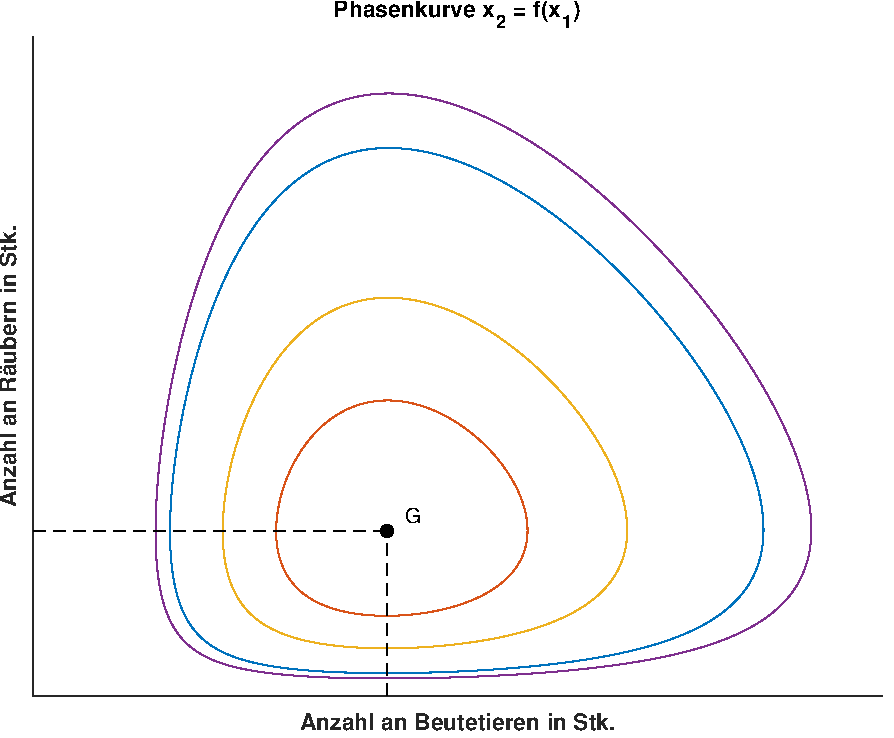
\includegraphics[width=0.6\linewidth,height=0.5\linewidth]{fig/exp/phaseG}
	\caption{Gleichgewichtslage in der Zustandsebene}
	\label{img:haupt:phaseG}
\end{figure}

Es ist anzumerken, dass die in \autoref{eqn:haupt:x1g} und \autoref{eqn:haupt:x2g} angegebenen Gleichgewichtslagen f�r $x_1$ und $x_2$ nicht von den Anfangspunkten abh�ngig sind. Diese Anfangspunkte bestimmen nur die entsprechende Trajektorie in der Zustandsebene. Die Ruhelage ist ausschlie�lich von den, in \autoref{sec:grundl:gl} genannten und beschriebenen, Faktoren $a_1, b_1, c_1, a_2,$ und $b_2$ abh�ngig. Diese beschreiben die entsprechenden Wechselwirkungen innerhalb und zwischen den Populationen. F�r die in \autoref{tab:haupt:param} gegebenen Werte, ergibt sich folgende Gleichgewichtslage:

\begin{align}
	x_{1G} &= \frac{b_2}{a_2} = \frac{0.1}{0.0002} = 500 \\
	x_{2G} &= \frac{(a_1 - b_1)}{c_1} = \frac{(0.05 - 0.02)}{0.0006} = 50
\end{align}

Eine M�glichkeit, die Gleichgewichtslage zu bestimmen, ist es diese numerisch zu approximieren. Hierzu wird in \autoref{lst:stat:code1} die Funktion $fsolve()$ verwendet. \autoref{eqn:haupt:statx12} und \autoref{eqn:haupt:statx22} werden, mit den entsprechenden Parametern $a_1, b_1, c_1, a_2$ und $b_2$, in einer anonymen Funktion gespeichert. Diese wird $fsolve()$ mit entsprechenden Startbedingungen �bergeben und anschlie�end die Gleichung $f = 0$ approximiert.

\begin{lstlisting}[style=Matlab-editor,caption={Verwenden von fsolve() f�r das numerische Bestimmen der Gleichgewichtslage},captionpos=b,label=lst:stat:code1,language=Matlab,basicstyle=\mlttfamily,numbers=none,frame=single,escapeinside={*@}{@*}]
% Parameter

% Beute / Hasen
a1 = 0.1; % Geburtenrate
b1 = 0.02; % Sterberate
c1 = 0.002; % Fressrate

% R�uber / F�chse
a2 = 0.0004; % Geburtenrate
b2 = 0.2; % Sterberate

% Deklarieren symbolischer Variablen
syms x1 x2
% Deklarieren der Gleichungen, um die Gleichgewichtslage zu bestimmen
f = @(x) [(a1 - b1 - c1*x(2));(a2*x(1) - b2)];
% Numerisches L�sen der Gleichungen mithilfe von vpasolve()
x = fsolve(f,[10,10])
\end{lstlisting}

Eine weitere M�glichkeit, die Gleichgewichtslage numerisch zu approximieren, ist mit der MATLAB Funktion $vpasolve()$ m�glich. In \autoref{lst:stat:code2} ist die Vorgehensweise hierzu exemplarisch dargestellt. In einem ersten Schritt werden hierbei die Parameter $a_1, b_1, c_1, a_2$ und $b_2$ deklariert und mit den in \autoref{tab:haupt:param} gegebenen Werten initialisiert. Anschlie�en werden, f�r die Zustandsvariablen $x_1$ und $x_2$, zwei symbolische Variablen mithilfe des \enquote{syms}-Befehls deklariert. Diese werden dazu verwendet, um \autoref{eqn:haupt:statx12} und \autoref{eqn:haupt:statx22}, unter Verwendung der symbolischen Variablen, in MATLAB zu definieren. Die definierten Gleichungen werden anschlie�end, mit der entsprechenden symbolischen Variablen, nach der die Gleichung aufgel�st werden soll, der Funktion $vpasolve()$ �bergeben. Diese approximiert numerisch N�herungswerte f�r $x_{1G}$ bzw. $x_{2G}$ und liefert die Ann�herungsl�sungen als R�ckgabewert.
\begin{lstlisting}[style=Matlab-editor,caption={Verwenden von vpasolve() f�r das numerische Bestimmen der Gleichgewichtslage},captionpos=b,label=lst:stat:code2,language=Matlab,basicstyle=\mlttfamily,numbers=none,frame=single,escapeinside={*@}{@*}]
% Parameter

% Beute / Hasen
a1 = 0.1; % Geburtenrate
b1 = 0.02; % Sterberate
c1 = 0.002; % Fressrate

% R�uber / F�chse
a2 = 0.0004; % Geburtenrate
b2 = 0.2; % Sterberate

% Deklarieren symbolischer Variablen
syms x1 x2
% Deklarieren der Gleichungen, um die Gleichgewichtslage zu bestimmen
eqnx1 = a1 - b1 - c1*x2 == 0;
eqnx2 = a2*x1 - b2 == 0;
% Numerisches L�sen der Gleichungen mithilfe von vpasolve()
% Erste Gleichung nach x2 aufl�sen
x2G = vpasolve(eqnx1, x2);
% Zweite Gleichung nach x1 aufl�sen
x1G = vpasolve(eqnx2, x1);
\end{lstlisting}

\FloatBarrier

\subsubsection{Einfluss eines einmaligen Eingriffs}
\label{sec:haupt:eingriff}
%Nachfolgend wird beschrieben, wie sich ein einmaliger Eingriff, beispielsweise durch Halbierung der R�uberpopulation, auf die Populationen auswirken kann. Dies ist beispielsweise eine wichtige Fragestellung in dem Bereich der Landwirtschaft. Hierbei k�nnen sch�dliche Insekten als Beute und Parasiten, die sich von den Insekten ern�hren, als R�uber interpretiert werden. Beide dieser Populationen sind Sch�dlinge, die in der Landwirtschaft bek�mpft werden. Hierbei stellt sich die Frage welcher Zeitpunkt, w�hrend des periodischen Bio-Zyklus, als g�nstig angesehen wird, um die Populationen zu verringern oder vernichten. Ein Eingreifen zu einem ung�nstigen Zeitpunkt kann die momentane Trajektorie in eine andere mit einer weitaus h�heren Schwankungen der Populationen transformieren. \cite[S. 35 f.]{lit:Foellinger1982}
\\
\\
Um einen passenden Zeitpunkt f�r die Sch�dlingsbek�mpfung treffen zu k�nnen, werden zun�chst die Phasenkurven in \autoref{img:haupt:phaseE} und die entsprechende Gleichgewichtslage analysiert. Die folgenden Geraden schneiden den station�ren Zustand und teilen die Zustandsebene in vier Subquadranten \cite[S. 7]{lit:Helmreich2011}:

\begin{align}
	x_2 &= \frac{(a_1 - b_1)}{c_1} 
	\label{eqn:haupt:x2E} \\
	x_1 &= \frac{a_2}{b_2}
	\label{eqn:haupt:x1E}
\end{align}

Der erste Subquadrant ist durch $x_2 \leq \frac{a_1 - b_1}{c_1}$ und $x_1 \leq \frac{a_2}{b_2}$ definiert. Dieser Teilbereich der Phasenkurven ist dadurch gekennzeichnet, dass sich die Anzahl an R�ubern $x_2$ verringert, w�hrend sich die Beutepopulation $x_1$ erh�ht. Eine Halbierung der R�uberpopulation $x_2$ hat hierbei die Transformation in eine Trajektorie mit einem gr��eren Umfang zur Folge. Die Schwankungen der beiden Populationen w�rden in diesem Fall zunehmen.
\\
\\
In dem zweiten Subquadranten gelten f�r $x_1 > \frac{a_2}{b_2}$ und $x_2 \leq \frac{a_1 - b_1}{c_1}$. Hierbei steigen beide Populationen an. \\Eine Halbierung der R�uber in diesem Subquadranten hat, wie im ersten Fall, eine Erh�hung der beiden Populationen zur Folge.
\\
\\
Der dritte Subquadrant ist durch $x_1 > \frac{a_2}{b_2}$ und $x_2 > \frac{a_1 - b_1}{c_1}$ definiert. Die Beutepopulation nimmt hierbei ab, w�hrend die R�uber sich vermehren. Eine Verringerung der R�uberpopulation hat, in diesem Fall, eine Verminderung beider Populationen zur Folge. Es erfolgt hierbei eine Transformation in eine der Gleichgewichtslage n�her gelegenen Trajektorie, die einen geringeren Umfang und somit geringere Schwankungen der Populationen aufweist. 
\\
\\
In dem vierten Subquadranten ist die Beutepopulation $x_1 \leq \frac{a_2}{b_2}$ und die Anzahl der R�uber $x_2 > \frac{a_1 - b_1}{c_1}$. In diesem Teilbereich verringern sich beide Populationen. Eine Verminderung der R�uber hat, wie f�r den dritten Subquadranten, eine Transformation in eine der Gleichgewichtslage n�her gelegenen Trajektorie zur Folge. Die Schwankungen der Populationen verringern sich ebenso f�r diesen Subquadranten.
\\
\\
Durch diese Fallunterscheidung l�sst sich auf einen g�nstigen Zeitpunkt schlie�en, um die R�uberpopulation dauerhaft zu verringern. Wenn diese bei einer Anzahl von $x_2 \geq 2 \cdot \frac{a_1 - b_1}{c_1}$ halbiert wird, resultiert dies in einer Transformation der momentanen Trajektorie in eine der Gleichgewichtslage n�her gelegenen Phasenkurve. Der neue Verlauf des Bio-Zyklus ist durch geringere Schwankungen der Populationen charakterisiert. Dies ist unabh�ngig von der aktuellen Beutepopulation $x_1$.

\begin{figure}
	\centering
	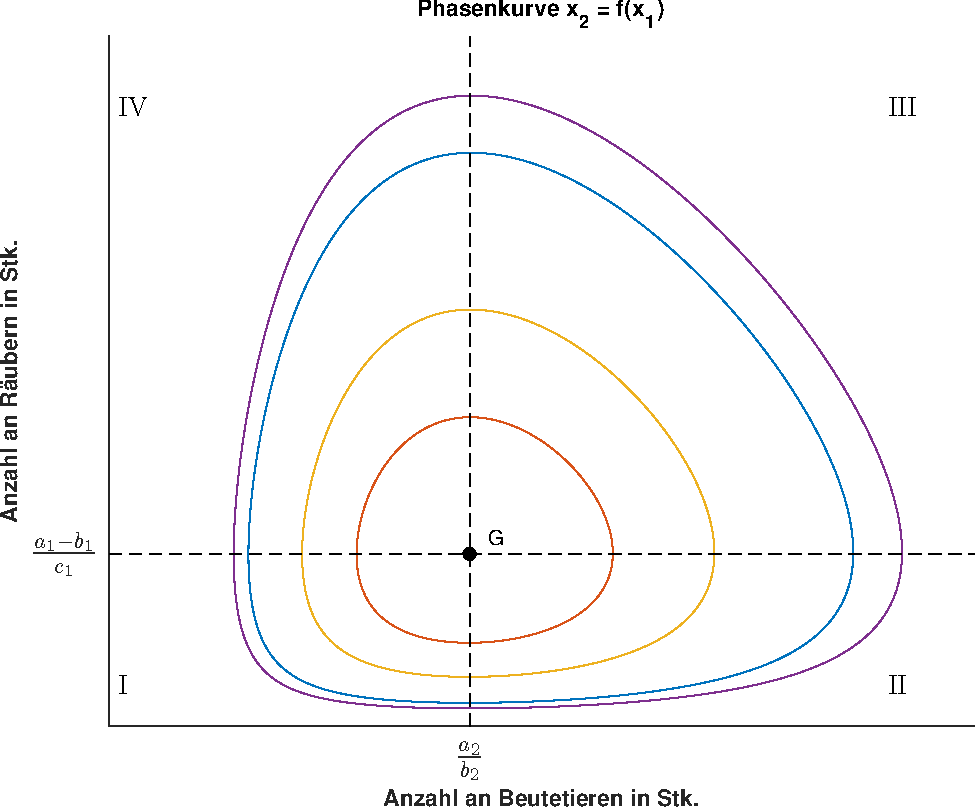
\includegraphics[width=0.6\linewidth,height=0.5\linewidth]{fig/exp/phaseE}
	\caption{Subquadranten der Trajektorien}
	\label{img:haupt:phaseE}
\end{figure}

In \autoref{img:haupt:eingriffs} sind die Auswirkungen eines Eingriffs, zu einem ung�nstigem Zeitpunkt, dargestellt. Eine Halbierung des Fuchsbestandes f�hrt hierbei zu einer Ver�nderung der Trajektorie. Die Transformation der Phasenkurve ist in \autoref{img:haupt:phaseEs} aufgezeigt. Die neue Trajektorie besitzt einen h�heren Umfang. Daraus folgt eine Zunahme an Schwankungen der Populationen. In \autoref{img:haupt:modellEs} sind diese dargestellt. Nach dem Eingriff sind gr��ere Amplituden w�hrend des periodischen Verlaufs zu vermerken.

\begin{figure}
	\begin{subfigure}[h]{0.49\linewidth}
		\centering
		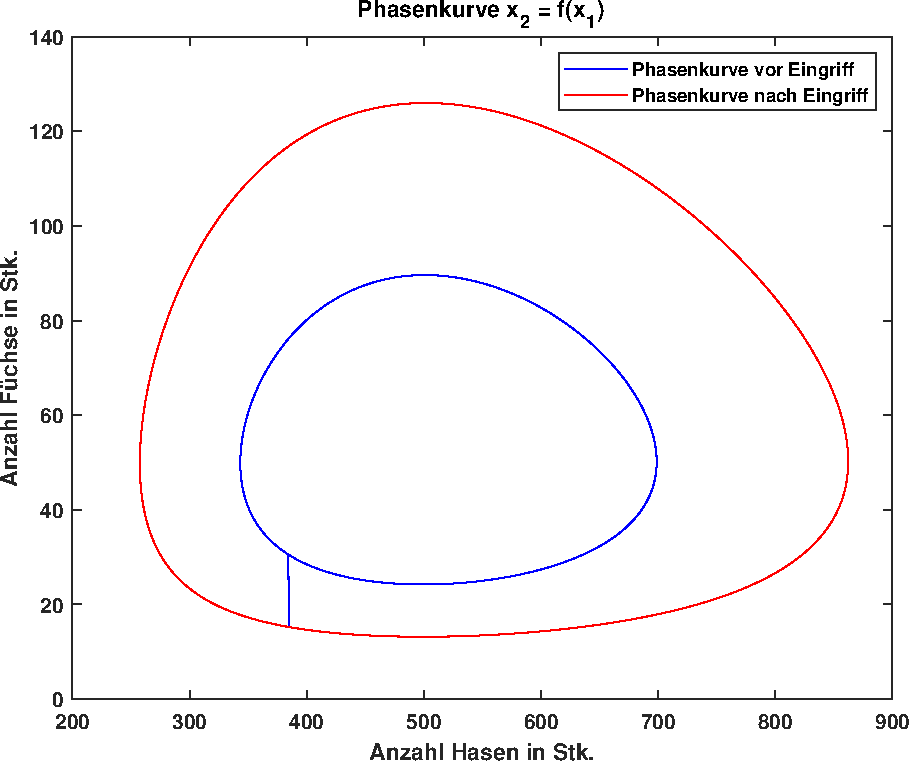
\includegraphics[width=\linewidth,height=0.8\linewidth]{fig/exp/phaseEs}
		\caption{Phasenkurve}
		\label{img:haupt:phaseEs}
	\end{subfigure}
	\hfill
	\begin{subfigure}[h]{0.49\linewidth}
		\centering
		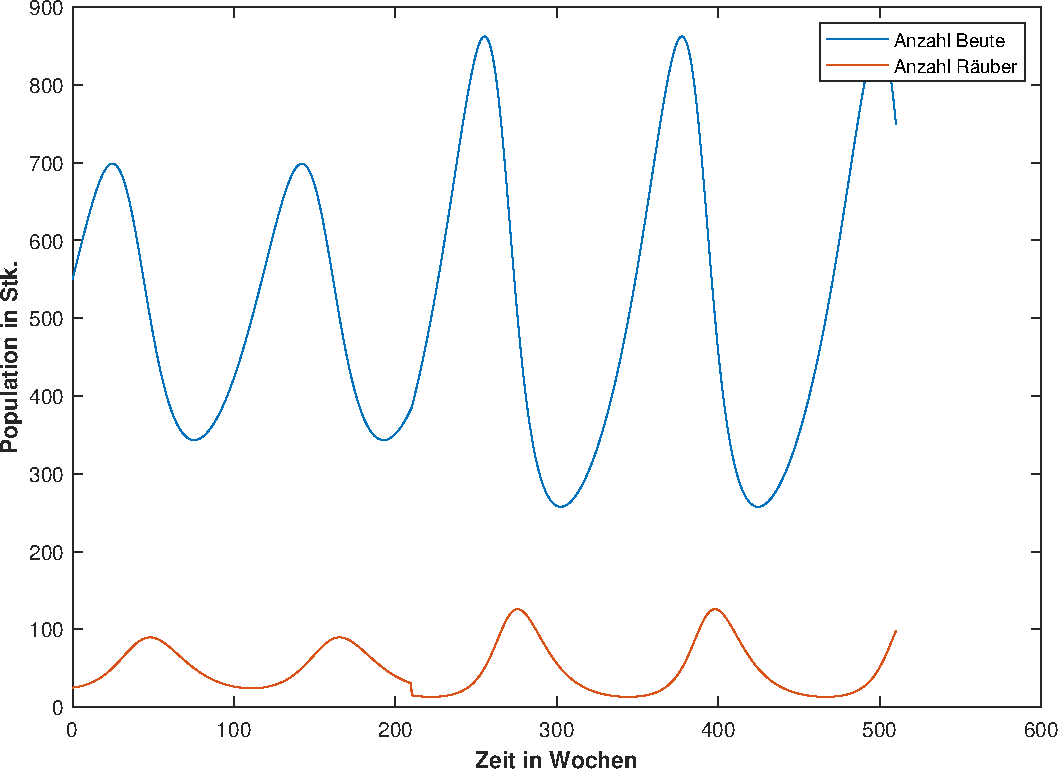
\includegraphics[width=\linewidth,height=0.8\linewidth]{fig/exp/modellEs}
		\caption{Verlauf der Populationen}
		\label{img:haupt:modellEs}
	\end{subfigure}
	\caption{Auswirkungen eines Eingriff zu einem ung�nstigem Zeitpunkt}
	\label{img:haupt:eingriffs}
\end{figure}

In \autoref{img:haupt:eingrifff} sind die gew�nschten Auswirkungen eines Eingriffs dargestellt. In \autoref{img:haupt:phaseEf} ist die Transformation in eine, der Gleichgewichtslage n�her gelegenen, Trajektorie zu erkennen. Daraus folgt ein stabilerer Verlauf der Populationen. Die Schwankungen bzw. Amplitude des periodischen Verlaufs ist hierbei, f�r beide Populationen, geringer.

\begin{figure}
	\begin{subfigure}[h]{0.49\linewidth}
		\centering
		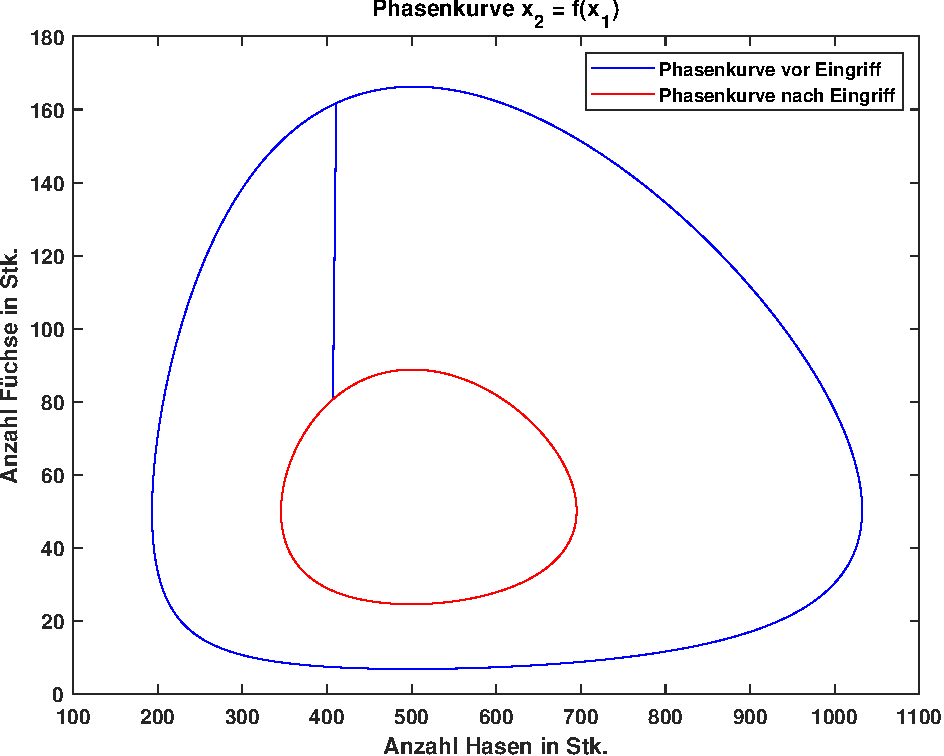
\includegraphics[width=\linewidth,height=0.8\linewidth]{fig/exp/phaseEf}
		\caption{Phasenkurve}
		\label{img:haupt:phaseEf}
	\end{subfigure}
	\hfill
	\begin{subfigure}[h]{0.49\linewidth}
		\centering
		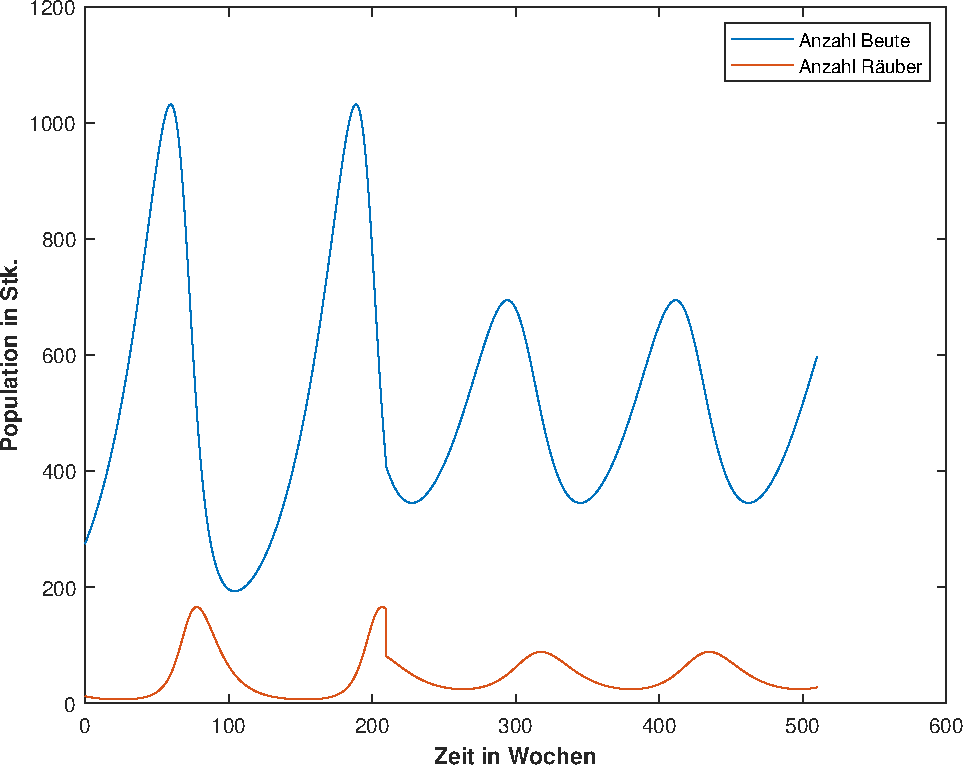
\includegraphics[width=\linewidth,height=0.8\linewidth]{fig/exp/modellEf}
		\caption{Verlauf der Populationen}
		\label{img:haupt:modellEf}
	\end{subfigure}
	\caption{Auswirkungen eines Eingriff zu einem g�nstigem Zeitpunkt}
	\label{img:haupt:eingrifff}
\end{figure}



\FloatBarrier
